\chapter{Конструкторский раздел}

\section{Схема базы данных}

На рисунке~\ref{chart:entities} представлена схема базы данных.

\begin{figure}[h]
    \centering
    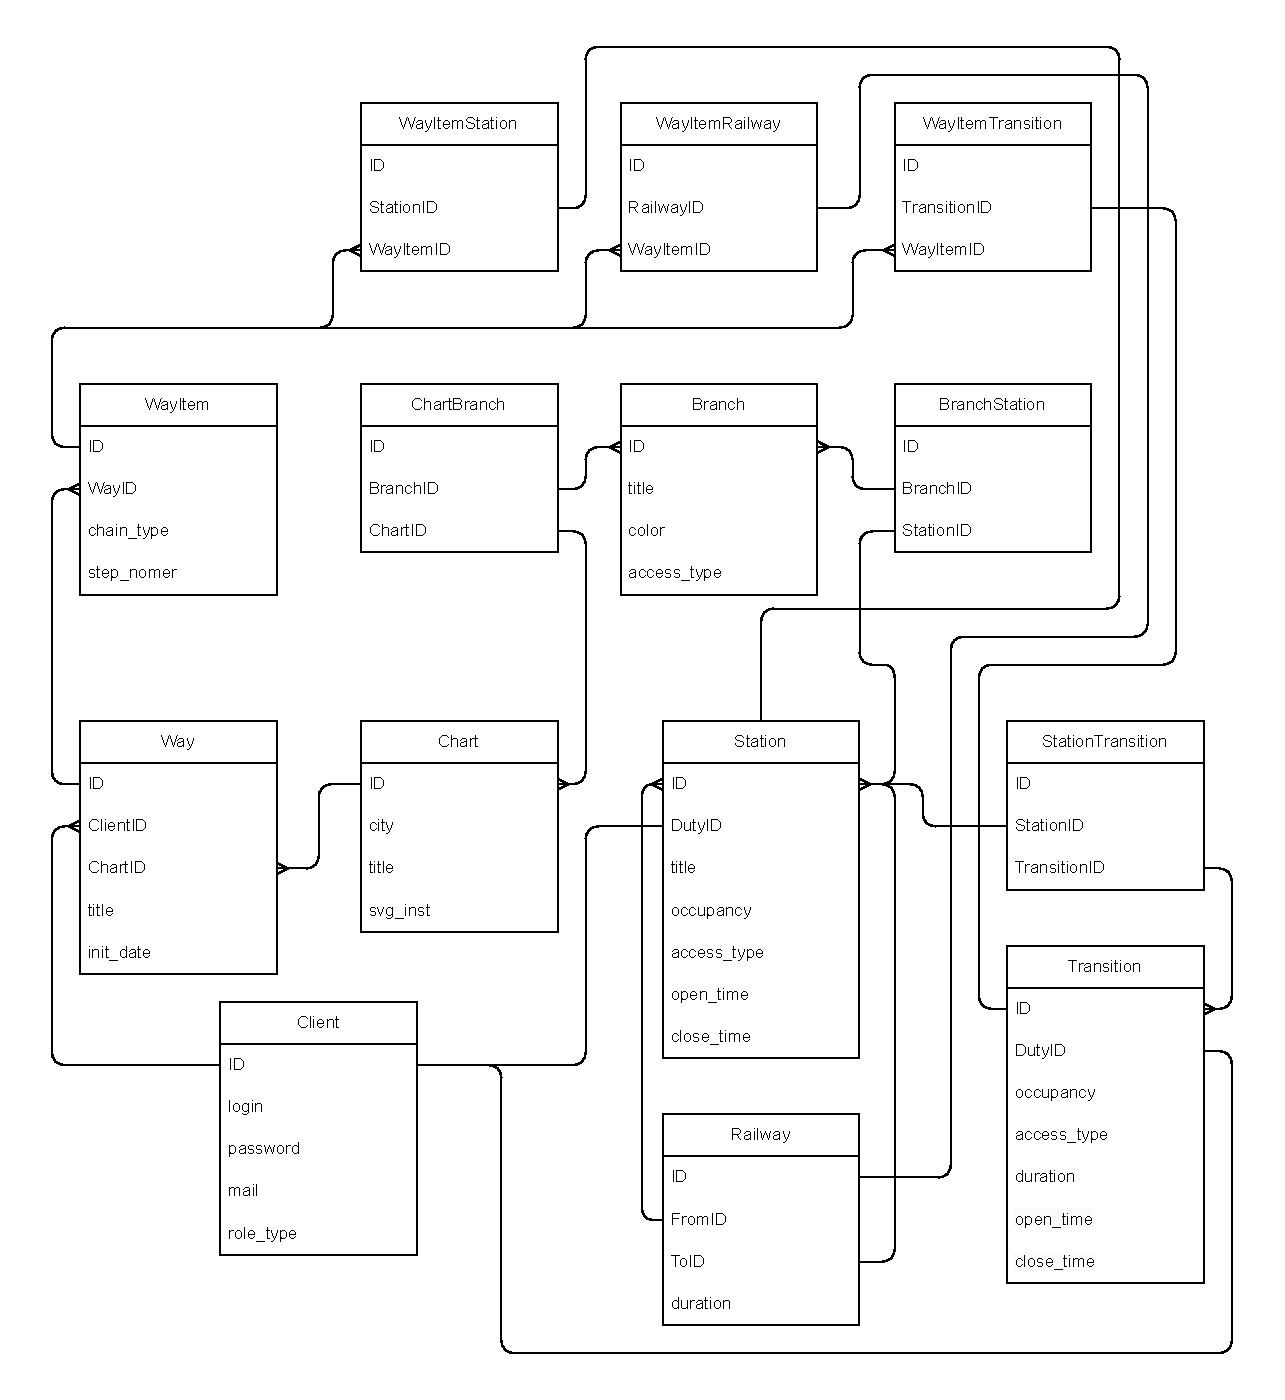
\includegraphics[width=\textwidth]{inc/img/Entities.pdf}
    \caption{Схема базы данных}
    \label{chart:entities}
\end{figure}

\FloatBarrier

\clearpage

\section{Описание сущностей базы данных}

Обозначения: PK --- первичный ключ, FK --- внешний ключ, U --- уникальное поле, NN --- обязательное для заполнения поле.

Описание сущностей базы данных приведено в таблицах~\ref{tbl:client}--\ref{tbl:way_item_transition}.

\begin{table}[H]
    \begin{center}
        \caption{Таблица client}
        \label{tbl:client}
        \begin{tabular}{|c|c|c|c|}
            \hline
            поле & тип данных & ограничения & значение \\
            \hline
            id & целое число & PK & идентификатор \\
            \hline
            client\_login & текст & NN, U & логин пользователя \\
            \hline
            password & текст & NN & защита \\
            \hline
            mail & дата и время & NN, U & уникальность клиента \\
            \hline
        \end{tabular}
    \end{center}    
\end{table}

\begin{table}[H]
    \begin{center}
        \caption{Таблица chart}
        \label{tbl:chart}
        \begin{tabular}{|c|c|c|c|}
            \hline
            поле & тип данных & ограничения & значение \\
            \hline
            id & целое число & PK & идентификатор пользователя \\
            \hline
            city & текст & NN, U & название города \\
            \hline
            title & текст & NN, U & название схемы \\
            \hline
            svg\_content & xml & NN & SVG представление схемы \\
            \hline
        \end{tabular}
    \end{center}    
\end{table}

\begin{table}[H]
    \begin{center}
        \caption{Таблица branch}
        \label{tbl:branch}
        \begin{tabular}{|c|c|c|c|}
            \hline
            поле & тип данных & ограничения & значение \\
            \hline
            id & целое число & PK & идентификатор \\
            \hline
            title & текст & NN, U & название ветки \\
            \hline
            color & целое число & NN & 10-e представление hex цвета \\
            \hline
            access & текст & NN & тип доступа \\
            \hline
        \end{tabular}
    \end{center}    
\end{table}

\begin{table}[H]
    \begin{center}
        \caption{Таблица station}
        \label{tbl:station}
        \begin{tabular}{|c|c|c|c|}
            \hline
            поле & тип данных & ограничения & значение \\
            \hline
            id & целое число & PK & идентификатор \\
            \hline
            duty\_id & целое число & FK & идентификатор дежурного \\
            \hline
            title & текст & NN, U & название станции \\
            \hline
            occupancy & целое число & NN & загруженность станции \\
            \hline
            access & текст & NN & тип доступа \\
            \hline
            open\_time & время без часового пояса & NN & время открытия станции \\
            \hline
            close\_time & время без часового пояса & NN & время открытия станции \\
            \hline
        \end{tabular}
    \end{center}    
\end{table}

\begin{table}[H]
    \begin{center}
        \caption{Таблица transition}
        \label{tbl:transition}
        \begin{tabular}{|c|c|c|c|}
            \hline
            поле & тип данных & ограничения & значение \\
            \hline
            id & целое число & PK & идентификатор \\
            \hline
            duty\_id & целое число & FK & идентификатор дежурного \\
            \hline
            occupancy & целое число & NN & загруженность станции \\
            \hline
            access & текст & NN & тип доступа \\
            \hline
            duration & Временной интервал & NN & среднее время перехода \\
            \hline
            open\_time & время без часового пояса & NN & время открытия перехода \\
            \hline
            open\_time & время без часового пояса & NN & время закрытия перехода \\
            \hline
        \end{tabular}
    \end{center}    
\end{table}

\begin{table}[H]
    \begin{center}
        \caption{Таблица railway}
        \label{tbl:ordering}
        \begin{tabular}{|c|c|c|c|}
            \hline
            поле & тип данных & ограничения & значение \\
            \hline
            id & целое число & PK & идентификатор \\
            \hline
            from\_id & целое число & NN, FK & связь с предыдущей станцией \\
            \hline
            to\_id & целое число & NN, FK & связь со следующей станцией \\
            \hline
            duration & Временной интервал & NN & среднее время переезда \\
            \hline
        \end{tabular}
    \end{center}    
\end{table}

\begin{table}[H]
    \begin{center}
        \caption{Таблица chart\_branch}
        \label{tbl:chart_branch}
        \begin{tabular}{|c|c|c|c|}
            \hline
            поле & тип данных & ограничения & значение \\
            \hline
            id & целое число & PK & идентификатор \\
            \hline
            chart\_id & целое число & NN, FK & идентификатор родительской схемы \\
            \hline
            branch\_id & целое число & NN, FK & идентификатор ветки \\
            \hline
        \end{tabular}
    \end{center}    
\end{table}

\begin{table}[H]
    \begin{center}
        \caption{Таблица branch\_station}
        \label{tbl:branch_station}
        \begin{tabular}{|c|c|c|c|}
            \hline
            поле & тип данных & ограничения & значение \\
            \hline
            id & целое число & PK & идентификатор \\
            \hline
            branch\_id & целое число & NN, FK & идентификатор родительской ветки \\
            \hline
            station\_id & целое число & NN, FK & идентификатор станции \\
            \hline
        \end{tabular}
    \end{center}    
\end{table}

\begin{table}[H]
    \begin{center}
        \caption{Таблица station\_transition}
        \label{tbl:branch_transition}
        \begin{tabular}{|c|c|c|c|}
            \hline
            поле & тип данных & ограничения & значение \\
            \hline
            id & целое число & PK & идентификатор \\
            \hline
            station\_id & целое число & NN, FK & идентификатор станции \\
            \hline
            transition\_id & целое число & NN, FK & идентификатор перехода \\
            \hline
        \end{tabular}
    \end{center}    
\end{table}

\begin{table}[H]
    \begin{center}
        \caption{Таблица way}
        \label{tbl:way}
        \begin{tabular}{|c|c|c|c|}
            \hline
            поле & тип данных & ограничения & значение \\
            \hline
            id & целое число & PK & идентификатор \\
            \hline
            client\_id & целое число & NN, FK & идентификатор пользователя \\
            \hline
            chart\_id & целое число & NN, FK & идентификатор схемы \\
            \hline
            title & текст & NN, U & название маршрута \\
            \hline
            duration & Временной интервал & NN & продолжительность маршрута \\
            \hline
            init\_date & Время с часовым поясом & NN & дата сохранения маршрута \\
            \hline
        \end{tabular}
    \end{center}    
\end{table}

\begin{table}[H]
    \begin{center}
        \caption{Таблица way\_item}
        \label{tbl:way_item}
        \begin{tabular}{|c|c|c|c|}
            \hline
            поле & тип данных & ограничения & значение \\
            \hline
            id & целое число & PK & идентификатор \\
            \hline
            way\_id & целое число & NN, FK & идентификатор родительского маршрута \\
            \hline
            nexus & текст & NN & тип связи \\
            \hline
            step\_nomer & целое число & NN & номер элемента звеня маршрута \\
            \hline
        \end{tabular}
    \end{center}    
\end{table}

\begin{table}[H]
    \begin{center}
        \caption{Таблица way\_item\_railway}
        \label{tbl:way_item_railway}
        \begin{tabular}{|c|c|c|c|}
            \hline
            поле & тип данных & ограничения & значение \\
            \hline
            id & целое число & PK & идентификатор \\
            \hline
            way\_item\_id & целое число & NN, FK & идентификатор родительского элемента маршрута \\
            \hline
            railway\_id & целое число & NN, FK & идентификатор переезда \\
            \hline
        \end{tabular}
    \end{center}    
\end{table}

\begin{table}[H]
    \begin{center}
        \caption{Таблица way\_item\_station}
        \label{tbl:way_item_station}
        \begin{tabular}{|c|c|c|c|}
            \hline
            поле & тип данных & ограничения & значение \\
            \hline
            id & целое число & PK & идентификатор \\
            \hline
            way\_item\_id & целое число & NN, FK & идентификатор родительского элемента маршрута \\
            \hline
            railway\_id & целое число & NN, FK & идентификатор станции \\
            \hline
        \end{tabular}
    \end{center}    
\end{table}

\begin{table}[H]
    \begin{center}
        \caption{Таблица way\_item\_transition}
        \label{tbl:way_item_transition}
        \begin{tabular}{|c|c|c|c|}
            \hline
            поле & тип данных & ограничения & значение \\
            \hline
            id & целое число & PK & идентификатор \\
            \hline
            way\_item\_id & целое число & NN, FK & идентификатор родительского элемента маршрута \\
            \hline
            railway\_id & целое число & NN, FK & идентификатор перехода \\
            \hline
        \end{tabular}
    \end{center}    
\end{table}

\section{Разработка триггеров}

Для поддержания целостности базы данных необходимо спроектировать спроектировать две группы триггеров:
\begin{enumerate}[label=\arabic*), labelsep=0.5em]
    \item триггеры поддерживающие целостность при обновлении или добавлении записей,
    \item триггеры поддерживающие целостность при удалении записей.
\end{enumerate}

На рисунках~\ref{alg:ch_trg}--\ref{alg:del_trg} представлены схемы триггеров.

\begin{figure}[h]
    \centering
    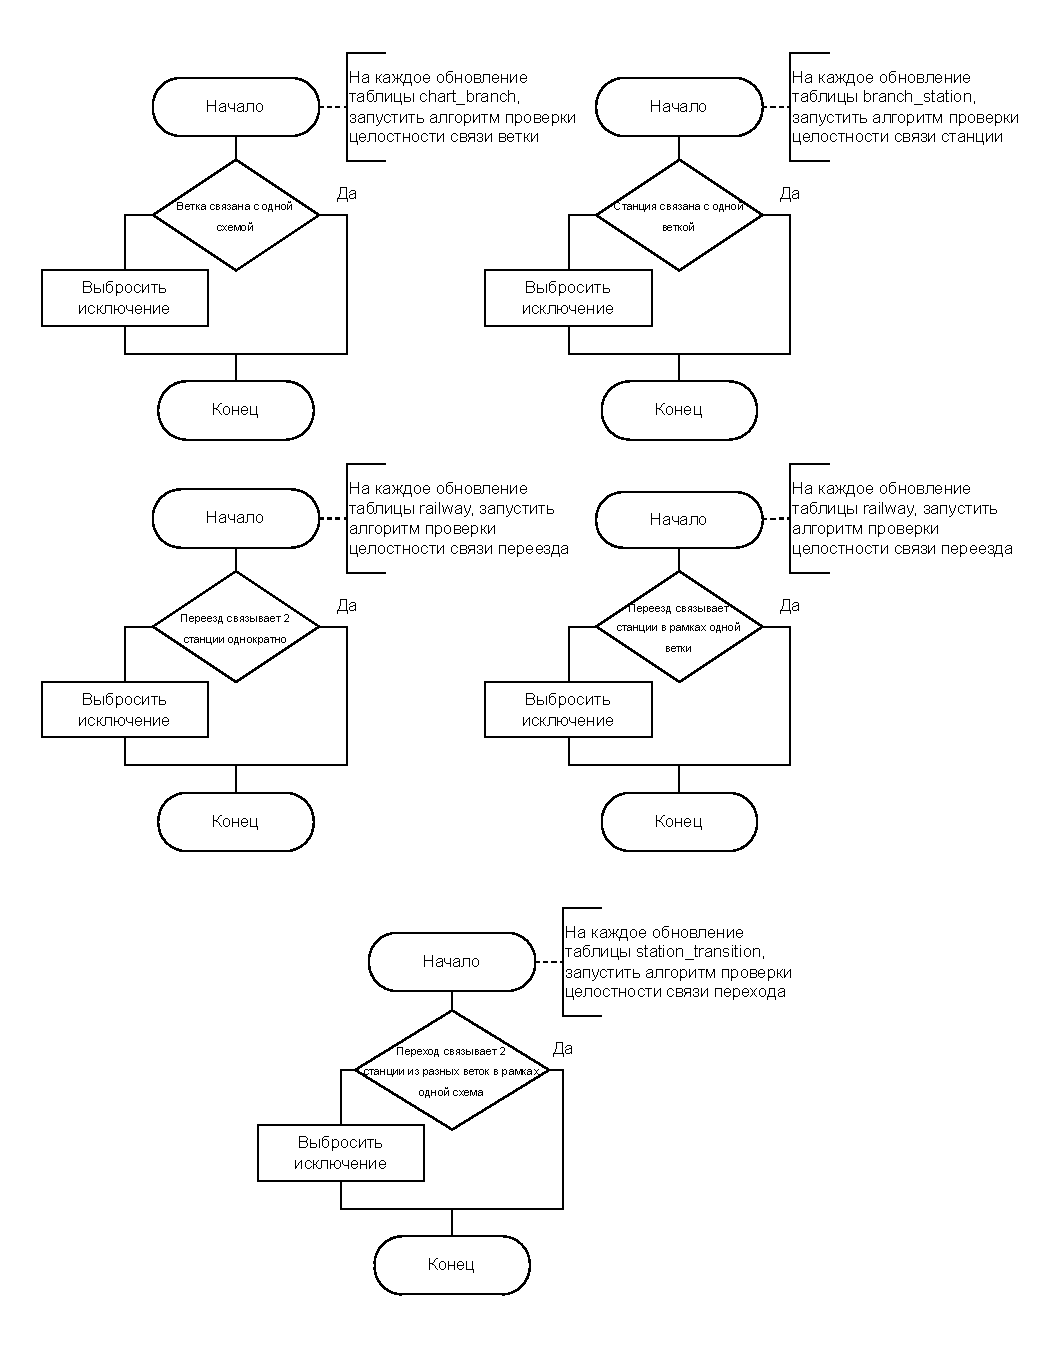
\includegraphics[width=\textwidth]{inc/img/ck_trg.pdf}
    \caption{Схема алгоритмов триггеров на обновления и добавления записей}
    \label{alg:ch_trg}
\end{figure}

\FloatBarrier

\begin{figure}[h]
    \centering
    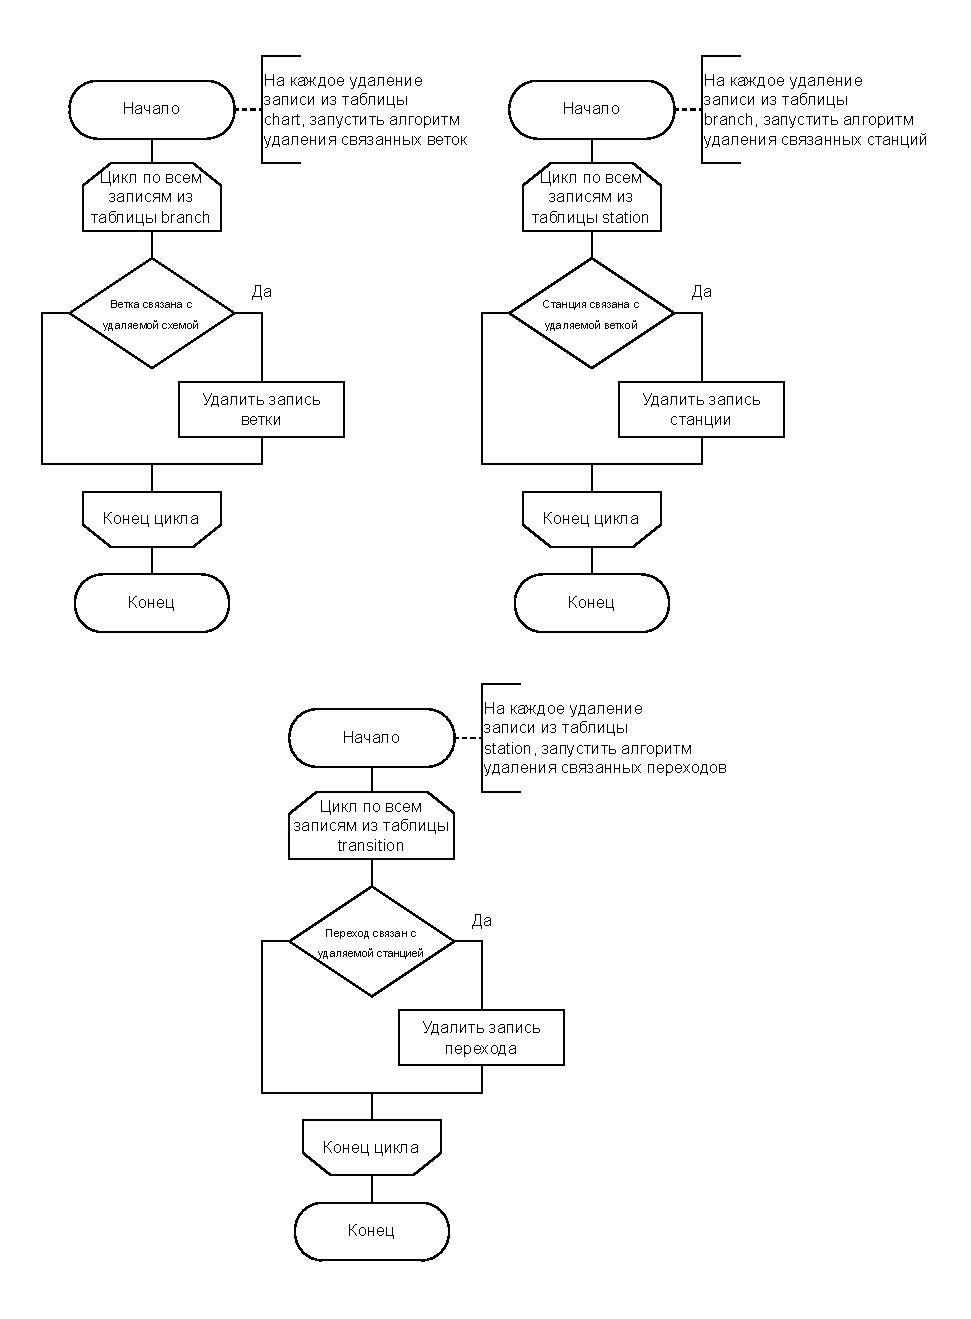
\includegraphics[width=\textwidth]{inc/img/del_trg.pdf}
    \caption{Схема алгоритмов триггеров на удаление записей}
    \label{alg:del_trg}
\end{figure}

\FloatBarrier

\section{Ролевая модель}
В данном разделе описаны права, которыми обладают пользователи на уровне базы данных.

Права неавторизованного пользователя:
\begin{itemize}
	\item[---] Чтение из таблиц client, chart, chart\_branch, branch, branch\_station, station, station\_transition, transition, railway;
	\item[---] вставка в таблицу client.
\end{itemize}

Права авторизованного пользователя:
\begin{itemize}
	\item[---] Чтение из таблиц client, chart, chart\_branch, branch, branch\_station, station, station\_transition, transition, railway, way, way\_item, way\_item\_railway, way\_item\_station, way\_item\_transition;
	\item[---] Вставка в таблицы client, way, way\_item, way\_item\_railway, way\_item\_station, way\_item\_transition.
\end{itemize}

Права дежурного:
\begin{itemize}
	\item[---] Чтение из таблиц client, chart, chart\_branch, branch, branch\_station, station, station\_transition, transition, railway, way, way\_item, way\_item\_railway, way\_item\_station, way\_item\_transition;
	\item[---] Вставка в таблицы client, station, railway, transition, way, way\_item, way\_item\_railway, way\_item\_station, way\_item\_transition.
\end{itemize}

Причем дежурный имеет доступ только к тем станциям переездам и переходам, которые связаны с ними по айди.
